%!TEX root = proj_report_outline.tex
\chapter{Implementation of the Web Application}

\section{Implementation Details}
The standard web application functionality required within the prototype, such as authentication, request life-cycles and password resets, was straightforward as Ruby on Rails solves many of these problems, and offers a wealth of libraries that can assist. The Pitch Card functionality and scope of disclosure functionality described in the Sections \ref{C:requirements} and \ref{C:design_web} were implemented from the ground up. In this Section these two functionality item's implementation details are explored.

\subsection{Pitch Card System}
As exemplified in Section \ref{C:requirements} Callaghan Innovation's specification for how the Pitch Card system works was quite mature and detailed. At it's core it required that users be able to initiate Pitch Cards and browse Pitch Cards, with the further ability to contribute suggestions or comments. To do this the web application separates the action's responsibilities. As discussed in Section \ref{SS:frameworkSelection} Ruby on Rails is architected on the MVC architecture pattern. Following Ruby on Rails convention the PitchHub prototype has models, views and controllers for each resource. The controllers adhere to the RESTful design principles, where resources are accessed using conventional HTTP resource methods and relationships are expressed via resource-nesting. The models, as designed in \ref{fig:class_diagram}, were implemented with the Mongoid \cite{Mongo4:online} Object Document Mapper (ODM) for MongoDB. The Mongoid ODM subscribes to the ``convention over configuration'' philosophy that is held highly in the Ruby on Rails framework, offering a simple façade over the MongoDB query language. The views were implemented with HTML, SASS (CSS), and JavaScript. To enhance the user experience AJAX was implemented to speed up page load times by loading secondary or non-essential data asynchronously. AJAX was also heavily used in user interactions, such as contributing a suggestion/comment and setting disclosure scopes (as an initiator).
\par
Figure \ref{fig:pitch_card_pitchhub} showcases the prototype's Pitch Card view from the initiator's perspective. The view can be deconstructed as follows: the sidebar contains the links to the main pages, the navigation bar contains the search box and user management dropdown, the main page space contains the Pitch Card and it's associated suggestions. Figure \ref{fig:dashboard_pitchhub} contains the same sidebar and navigation bar however the main page space contains a grid of mini-pitch card views consisting of the Pitch Card's image (if any) as well as the \textit{Value Proposition} pitch point.

\subsection{Scope of Disclosure}
As 

\section{Implementation Challenges}

\section{Virtualised Development Environment}

\section{Deployment}


\begin{sidewaysfigure}[ht]
    \centering
    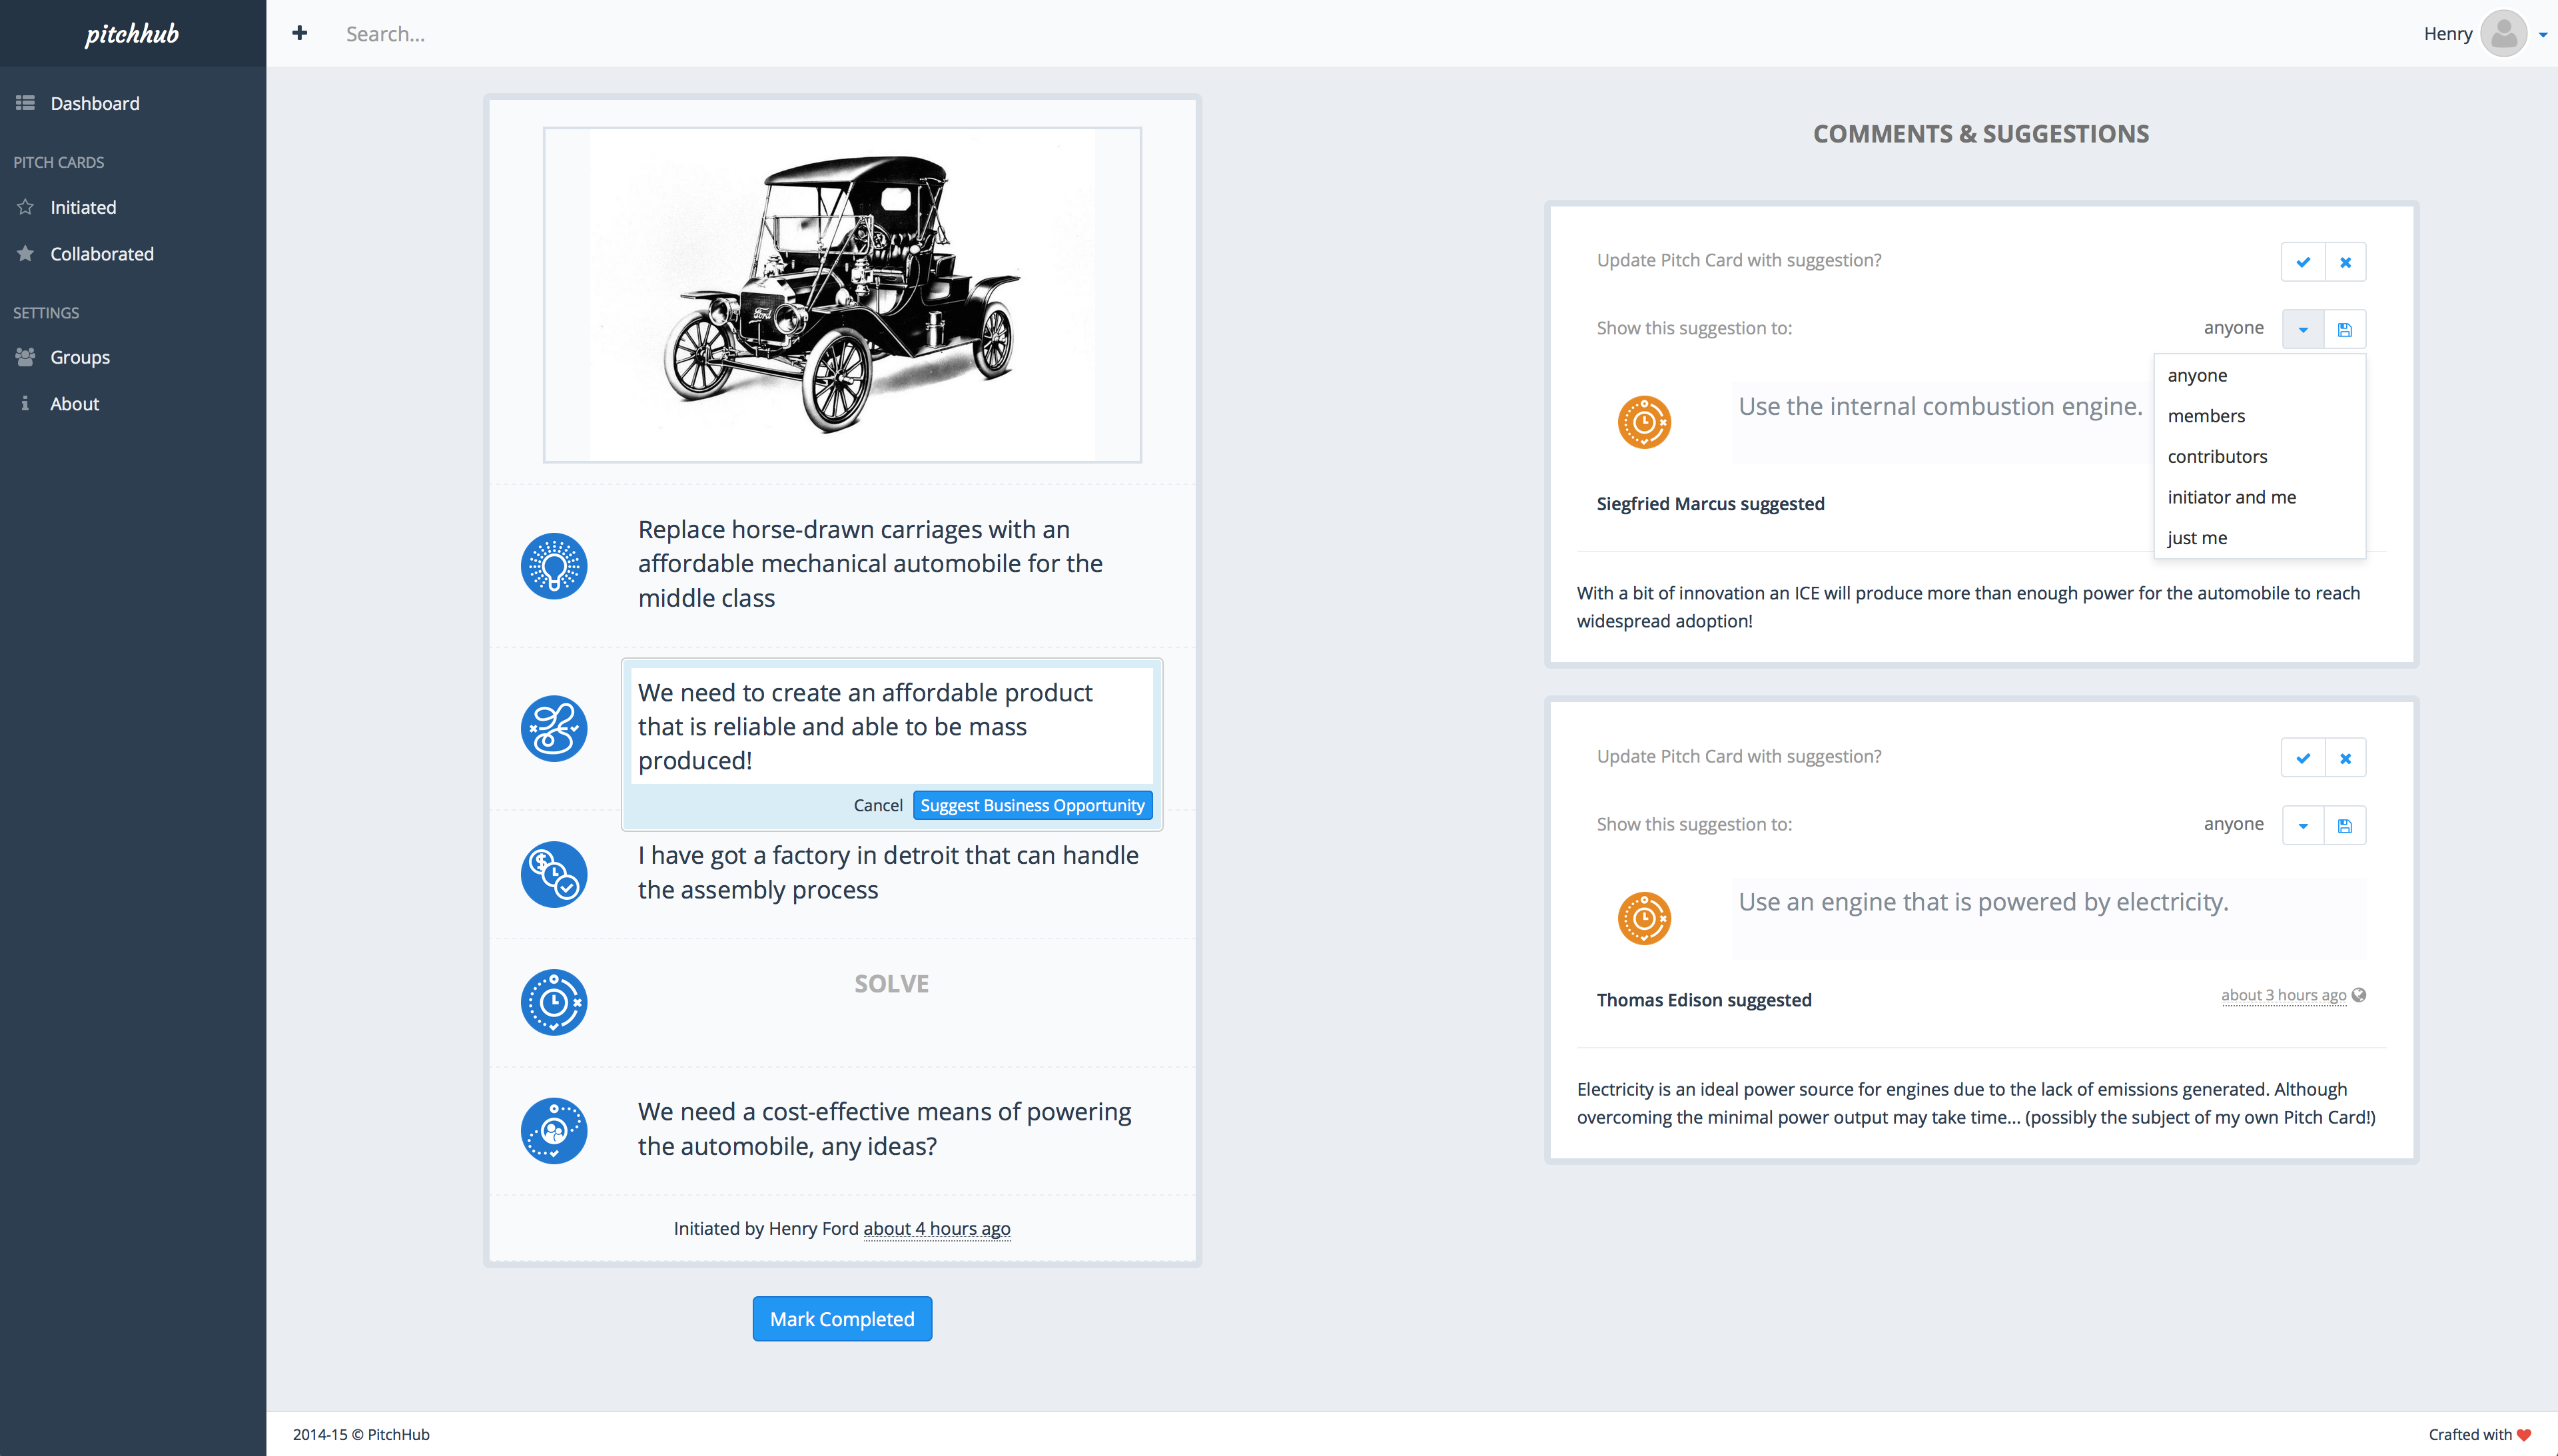
\includegraphics[width=1\textwidth]{pitch_card_pitchhub}
    \caption{Fictional Ford Model T Pitch Card view from the initiator's perspective. The view is divided into two sections the Pitch Card and it's suggestions/comments. In the Pitch Card half users perform in-line editing on a Pitch Point to make a suggestion. In the suggestion/comments half the initiator may accept or decline the suggestion and set the suggestion/comment's scope.}
    \label{fig:pitch_card_pitchhub}
\end{sidewaysfigure}

\begin{sidewaysfigure}[ht]
    \centering
    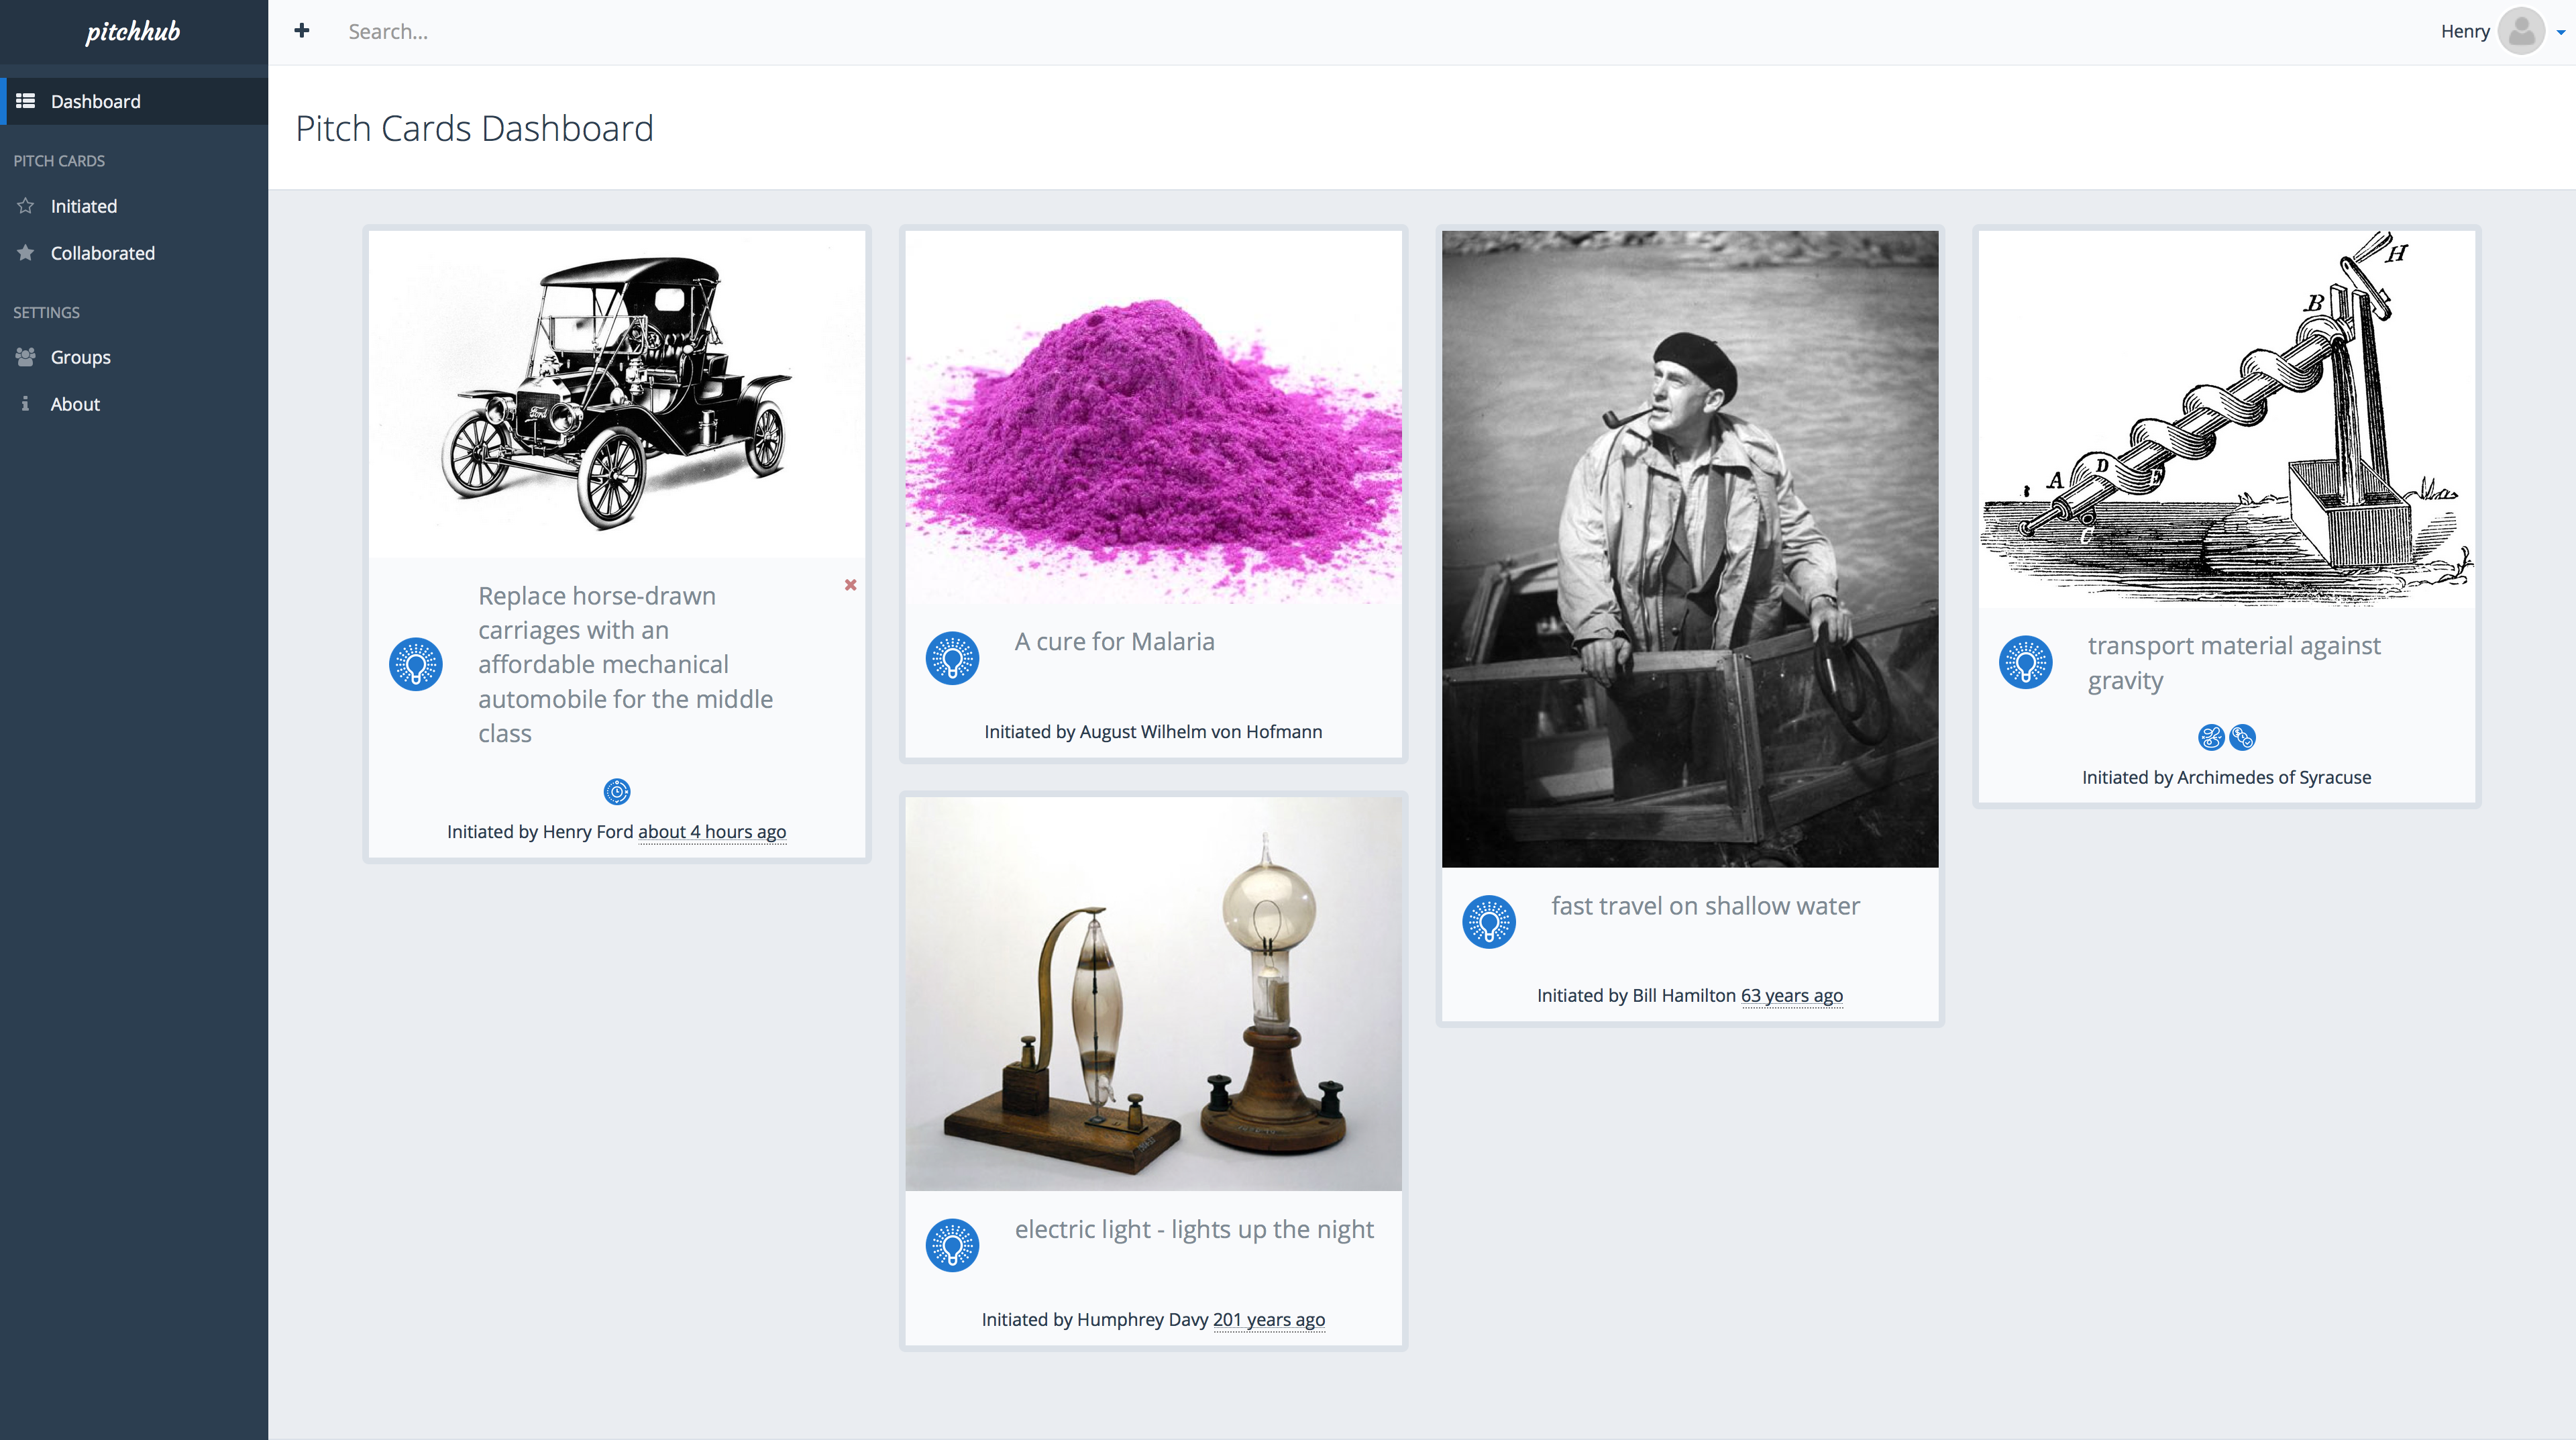
\includegraphics[width=1\textwidth]{dashboard_pitchhub}
    \caption{PitchHub's dashboard populated with fictional Pitch Cards. The grid layout displayed is responsive, so the Pitch Cards will reorganise and size to fit the user's device screen.}
    \label{fig:dashboard_pitchhub}
\end{sidewaysfigure}